\section{Experiments}

\subsection{Training Details}
In this work we enhanced the model's mathematical performance by introducing various modifications to the PPO algorithm based on the Qwen-32B model. These techniques are also effective for other reasoning tasks, such as code-related tasks. For the basic PPO, we used AdamW as the optimizer, setting the actor learning rate to \(1 \times 10^{-6}\) and the critic learning rate to \(2 \times 10^{-6}\), as the critic needs to update faster to keep pace with policy changes. The learning rate employed a warmup-constant scheduler. The batch size was 8192 prompts, with each prompt sampled once, and each mini-batch size set to 512. The value network was initialized using a reward model, with the GAE $\lambda$ set to 0.95 and $\gamma$ set to 1.0. Sample-level loss was used, and the clip $\epsilon$ was set to 0.2.

Compared to vanilla PPO, VAPO made the following parameter adjustments:
\begin{enumerate}
\item Implemented a value network warmup for 50 steps based on the reward model (RM) before initiating policy training.
\item Utilized decoupled GAE, where the value network learns from returns estimated with $\lambda$=1.0, while the policy network learns from advantages obtained using a separate lambda.
\item Adaptively set the lambda for advantage estimation based on sequence length, following the formula: $\lambda_{\text{policy}} = 1-\frac{1}{\alpha l}$, where $\alpha=0.05$.
\item Adjusted the clip range to $\epsilon_\text{high}$=0.28 and $\epsilon_
\text{low}$=0.2.
\item Employed token-level policy gradient loss.
\item Added a positive-example language model (LM) loss to the policy gradient loss, with a weight of 0.1.
\item Used 512 prompts per sampling, with each prompt sampled 16 times, and set the mini-batch size to 512.
\end{enumerate}

We will also demonstrate the final effects of removing each of these seven modifications from VAPO individually. For the evaluation metric, we use the average pass rate of AIME24 over 32 times, with sampling parameters set to topp=0.7 and temperature=1.0.


\subsection{Ablation Results}


\setcounter{table}{0}
\begin{table}[t]
    \centering
    \caption{Abalation results of \textbf{VAPO}}
    \begin{tabular}{l c}
        \toprule
        \textbf{Model} & $\textbf{AIME24}_\text{avg@32}$ \\
        \midrule
        Vanilla PPO & 5 \\
        \textbf{DeepSeek-R1-Zero-Qwen-32B}  & 47 \\
        \textbf{DAPO} & 50 \\
        \midrule
        VAPO w/o Value-Pretraining & 11 \\
        VAPO w/o Decoupled-GAE & 33 \\
        VAPO w/o Length-adaptive GAE & 45 \\
        VAPO w/o Clip-Higher & 46 \\
        VAPO w/o Token-level Loss & 53 \\
        VAPO w/o Positive Example LM Loss & 54 \\
        VAPO w/o Group-Sampling & 55 \\
        \textbf{VAPO} & \textbf{60} \\
        \bottomrule
    \end{tabular}
    \label{tab:results}
\end{table}


On Qwen-32b, DeepSeek R1 using GRPO achieves 47 points on AIME24, while DAPO reaches 50 points with 50\% of the update steps. In Figure~\ref{fig:front}, our proposed VAPO matches this performance using only 60\% of DAPO's steps and achieves a new SOTA score of 60.4 within just 5,000 steps, demonstrating VAPO's efficiency. Additionally, VAPO maintains stable entropy—neither collapsing nor becoming excessively high—and consistently achieves peak scores of 60-61 across three repeated experiments, highlighting the reliability of our algorithm.

\Cref{tab:results} systematically presents our experimental results. The Vanilla PPO method, hindered by value model learning collapse, only achieves 5 points in the later stages of training, characterized by a drastic reduction in response length and the model directly answering questions without reasoning.
Our VAPO method finally achieves 60 points, which is a significant improvement. We further validated the effectiveness of the seven proposed modifications by ablating them individually:
\begin{enumerate}
\item Without Value-Pretraining, the model experiences the same collapse as Vanilla PPO during training, converging to a maximum of approximately 11 points.
\item Removing the decoupled GAE causes reward signals to exponentially decay during backpropagation, preventing the model from fully optimizing long-form responses and leading to a 27-point drop.
\item Adaptive GAE balances optimization for both short and long responses, yielding a 15-point improvement.
\item Clip higher encourages thorough exploration and exploitation; its removal limited the model's maximum convergence to 46 points.
\item Token-level loss implicitly increased the weight of long responses, contributing to a 7-point gain.
\item Incorporating positive-example LM loss boosted the model by nearly 6 points.
\item Using Group-Sampling to generate fewer prompts but with more repetitions also resulted in a 5-point improvement.
\end{enumerate}

\subsection{Training Dynamics}

\begin{figure}[t]
    \centering
    \begin{subfigure}{0.45\textwidth}
        \centering
        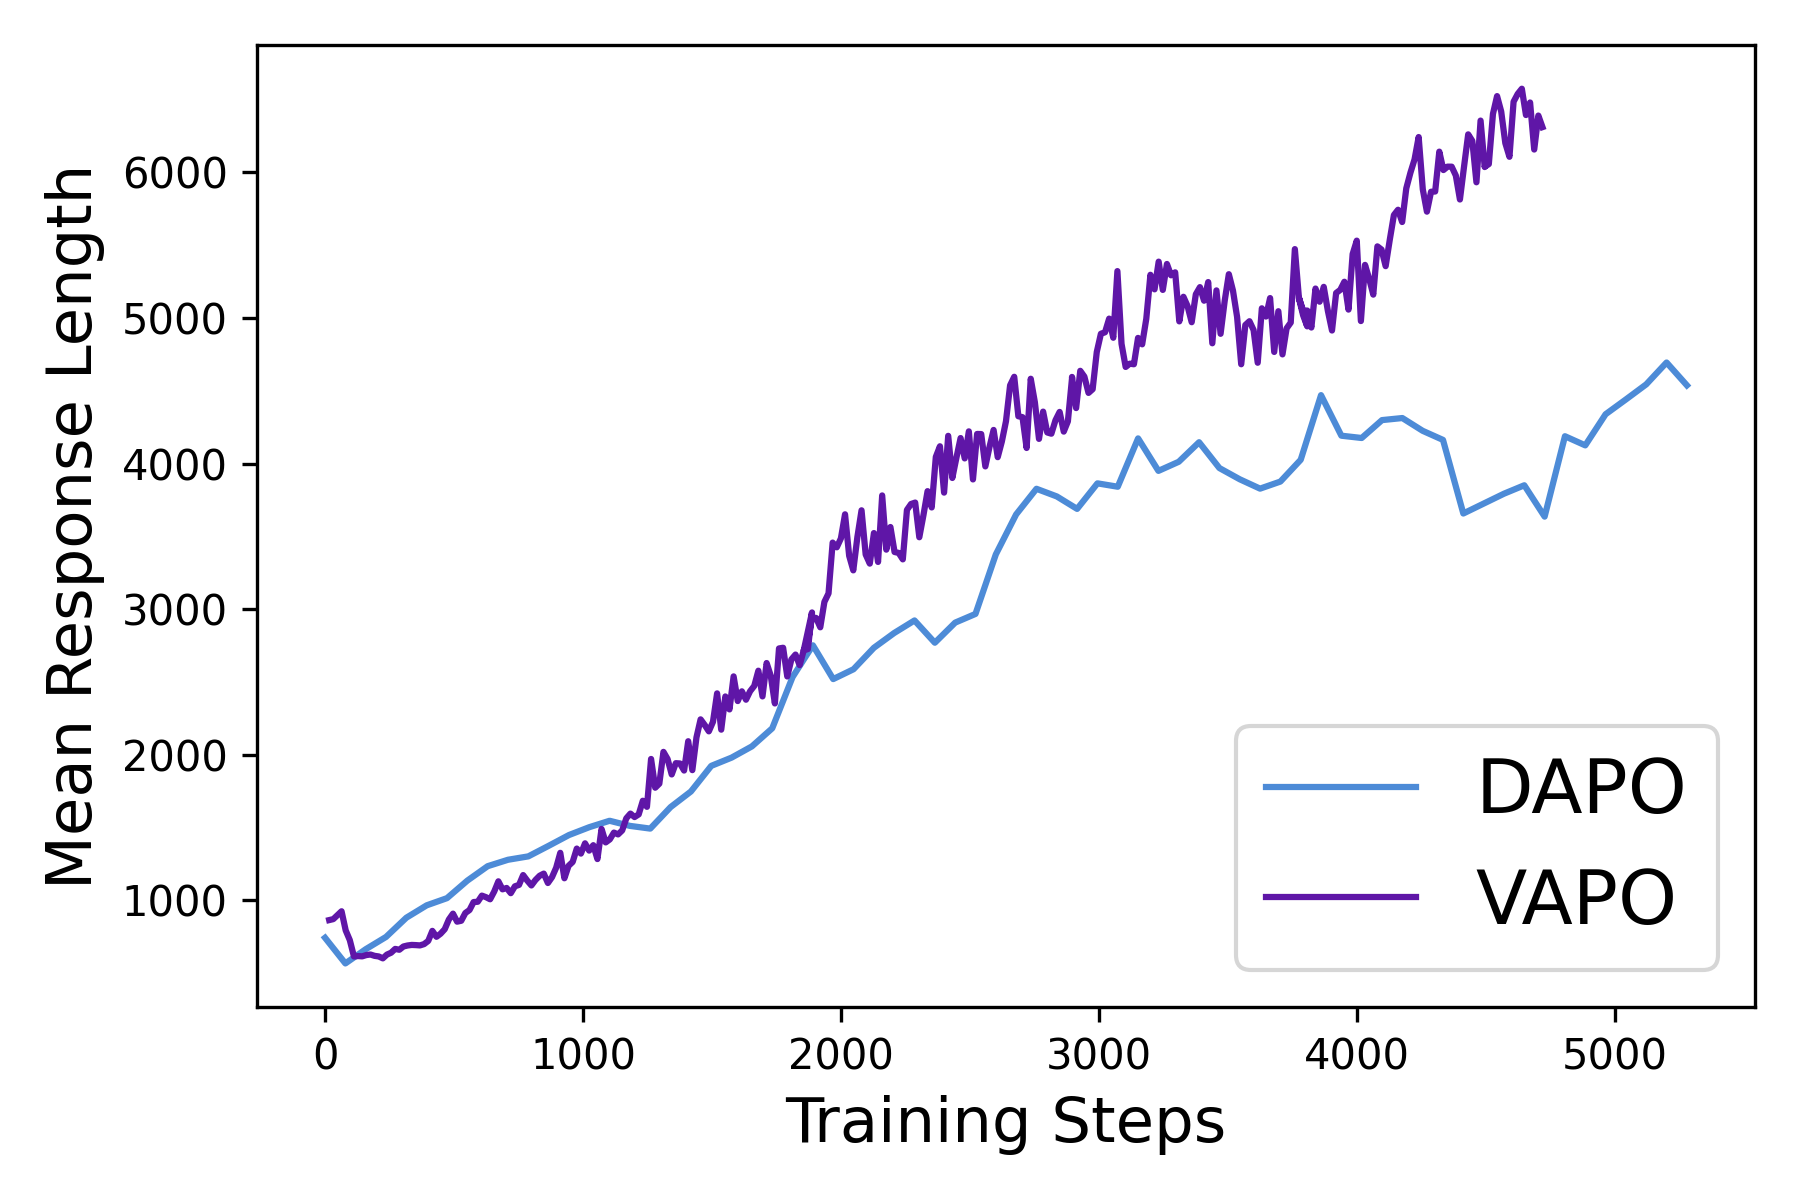
\includegraphics[width=\textwidth]{fig/length.png}
        % \captionsetup{labelformat=empty} % 只显示编号,不显示标题
        \caption{Mean response length.}
        \label{subfig:length}
    \end{subfigure}
    \begin{subfigure}{0.45\textwidth}
        \centering
        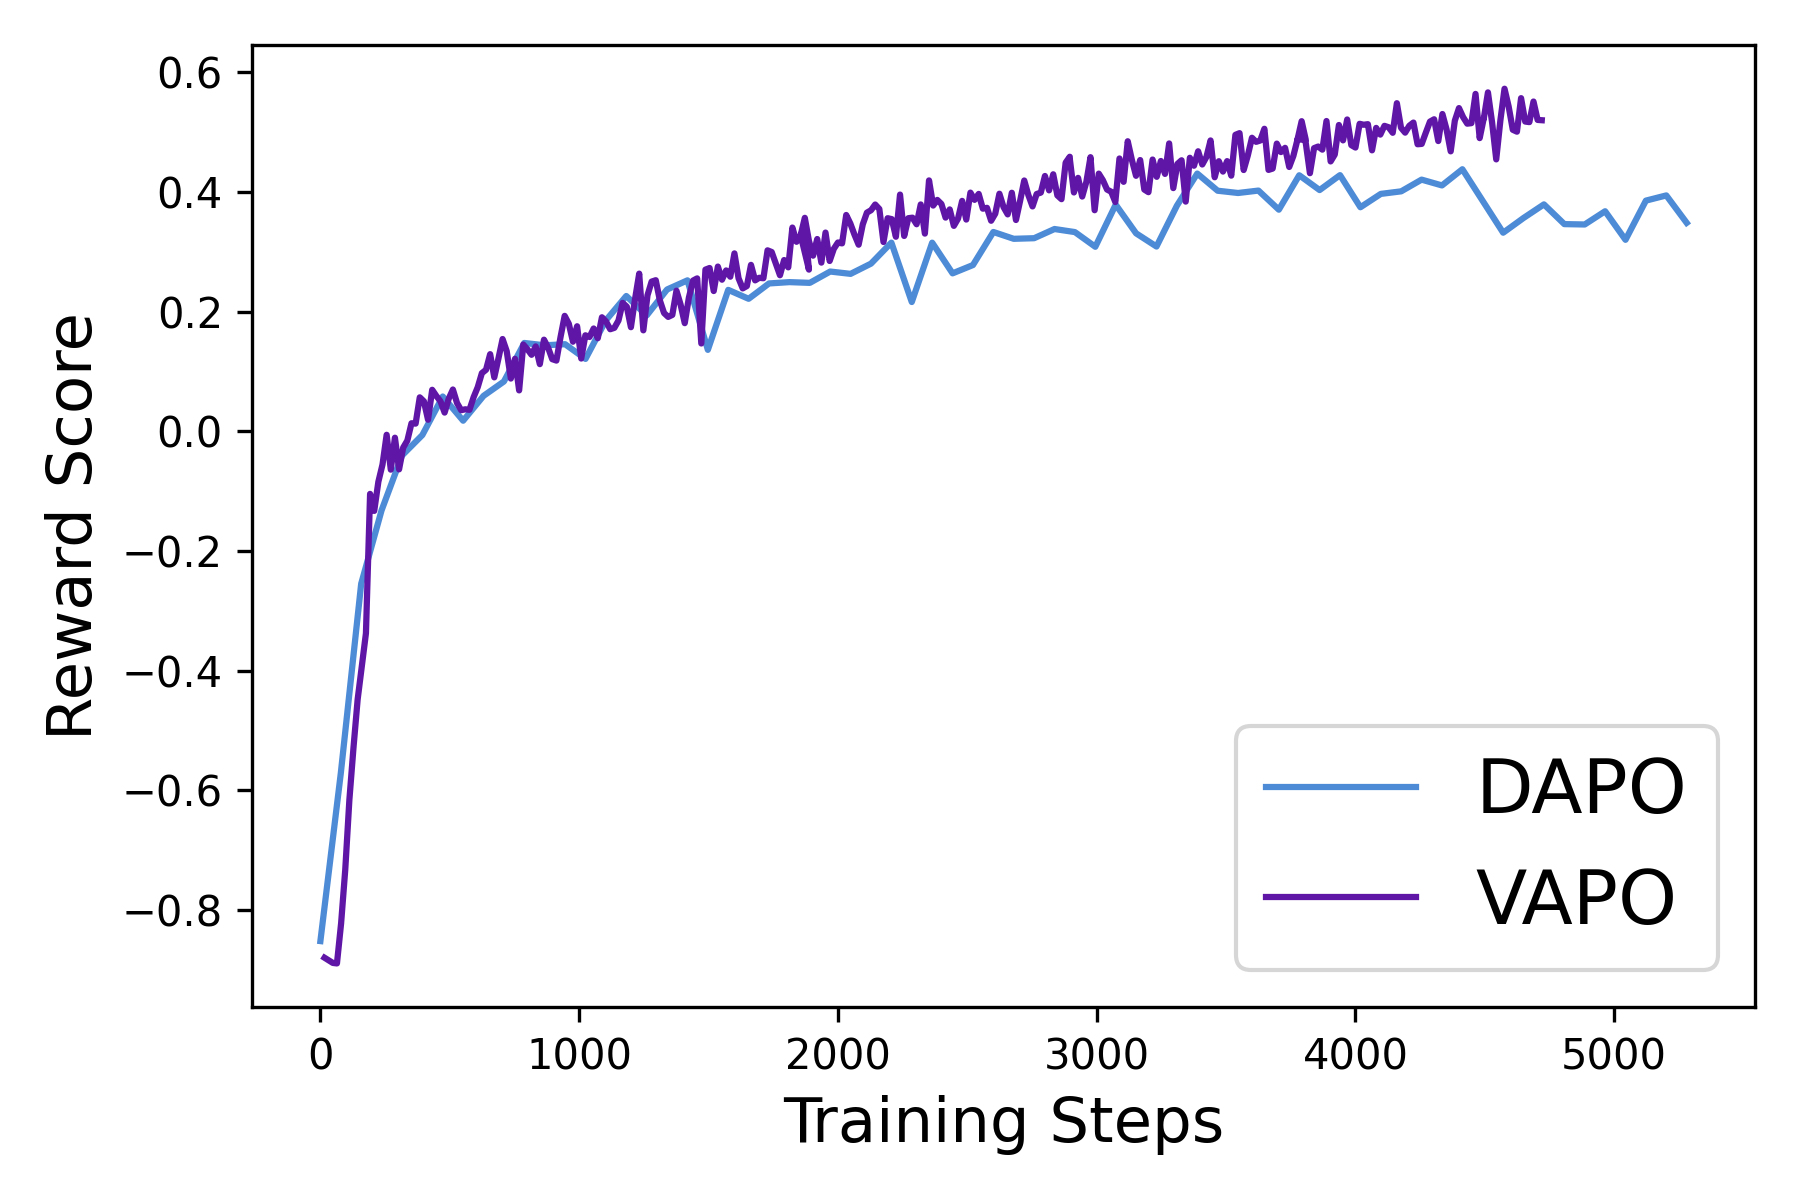
\includegraphics[width=\textwidth]{fig/reward.png}
        % \captionsetup{labelformat=empty} % 只显示编号,不显示标题
        \caption{Reward score.}
        \label{subfig:reward}
    \end{subfigure}
    \begin{subfigure}{0.45\textwidth}
        \centering
        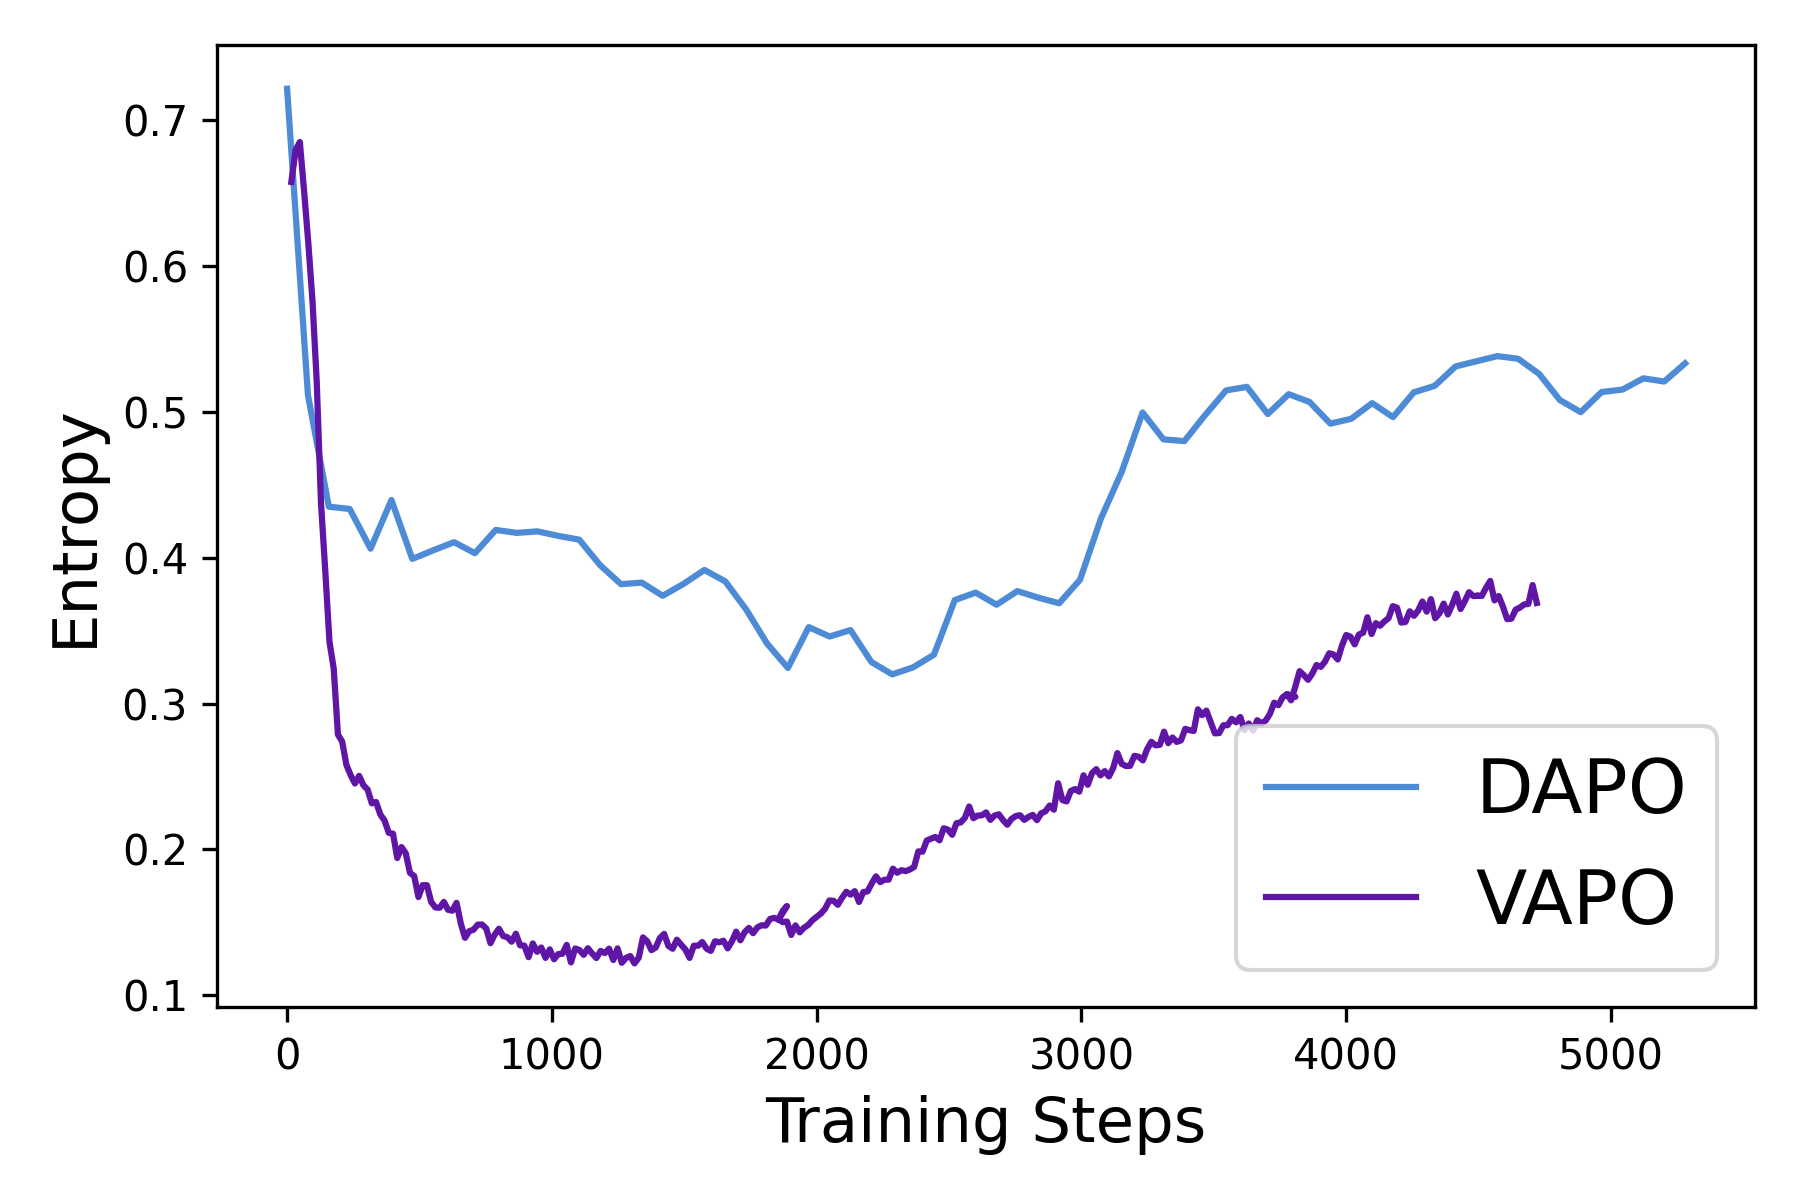
\includegraphics[width=\textwidth]{fig/entropy.png}
        % \captionsetup{labelformat=empty} % 只显示编号,不显示标题
        \caption{Generation entropy.}
        \label{subfig:entropy}
    \end{subfigure}
    \caption{VAPO's metric curves for response length, reward score, and generation entropy.}
    \label{fig:metrics}
\end{figure}

The curves generated during RL training provide real-time insights into training stability, and comparisons between different curves can highlight algorithmic differences. It is generally believed that smoother changes and faster growth are the desirable characteristics of these curves. Through a comparison of the training processes of VAPO and DAPO, we made the following observations:
\begin{itemize}
\item \Cref{fig:metrics} shows that VAPO's training curve is smoother than DAPO's, indicating more stable algorithmic optimization in VAPO.
\item As depicted in \Cref{subfig:length}, VAPO exhibits superior length scaling compared to DAPO. In modern contexts, better length scaling is widely recognized as a marker of improved model performance, as it enhances the model's generalization capabilities.
\item \Cref{subfig:reward} demonstrates that VAPO's score grows faster than DAPO's, as the value model provides the model with more granular signals to accelerate optimization.
\item According to \Cref{subfig:entropy}, VAPO's entropy drops lower than DAPO's in the later stages of training. This is two sides of the coin: on one hand, it may hinder exploration, but on the other hand, it improves the model stability. From VAPO's final results, the lower entropy has minimal negative impact on performance, while the reproducibility and stability proves highly advantageous.
\end{itemize}
